\documentclass{article}
\usepackage{graphicx} % Required for inserting images
\usepackage[rightcaption]{sidecap}
\usepackage[style=alphabetic]{biblatex}

\graphicspath{ {./images/} }
\addbibresource{sample.bib}

\title{Assignment 4 Report}
\author{Ole Rößler (7211)}
\date{December 2024}

\begin{document}

\maketitle
\tableofcontents

\newpage
\section{Design Exercise: Flight Booking System}

\subsection{Requirements}
This will talk about functional and non-functional requirements of the system given by the.
The main points given were about the given points considering (this will be a short overview about the task).

Short Description what the differences between function and non-function requirements are and I chose them (from the given context and my personal thought).

\subsubsection{Functional Requirements}
\paragraph{Booking}
TODO
\paragraph{View Prices}
TODO
\paragraph{Fetching Data}
TODO
\paragraph{Price Consistency}
TODO

\subsubsection{Non-Functional Requirements}
\paragraph{Usability}
TODO\paragraph{Speed}
TODO
\subsection{System Architecture}
TODO
\begin{figure}[h]
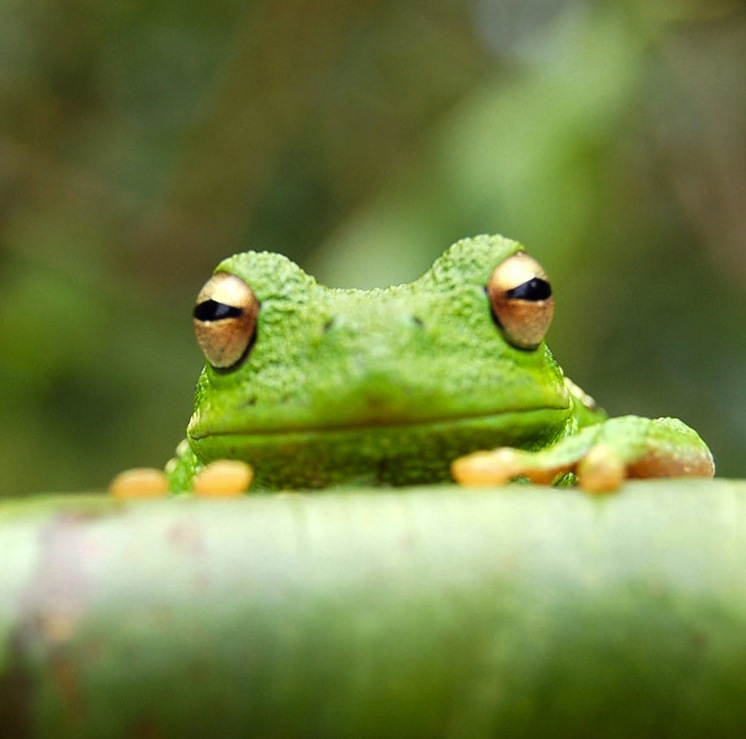
\includegraphics[width=\textwidth]{frog.jpg}
\caption{Design of my architecture}
\end{figure}
TODO

\subsection{Discussion}
TODO

\printbibliography[heading=bibintoc]
\end{document}
